\section{Additional Figures}

\steve{This section title will change and is just a placeholder for now.}

\begin{figure}
  \centering
  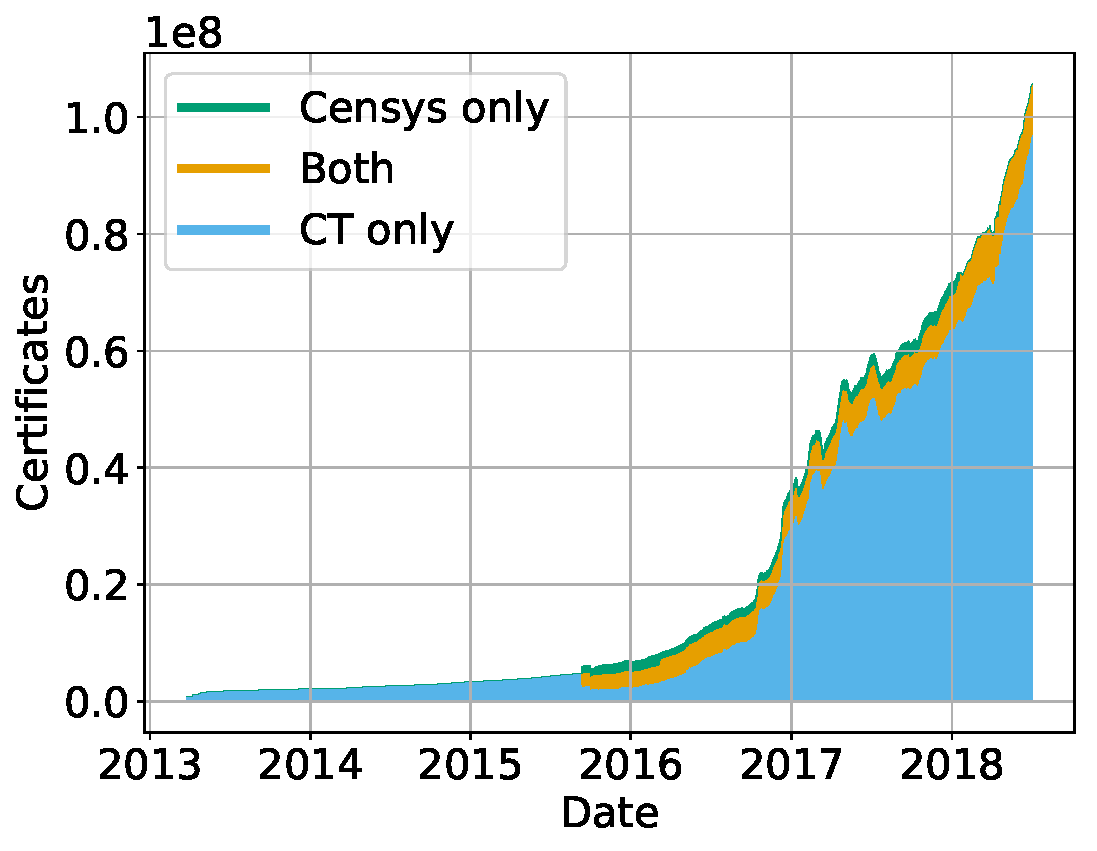
\includegraphics[width=\linewidth]{fig/cert_count_valid}
  \caption{Number of unique certificates seen by Censys and \ac{ct} over time.}
  \label{fig:count:certs}
\end{figure}

\begin{figure}[t]
  \centering
  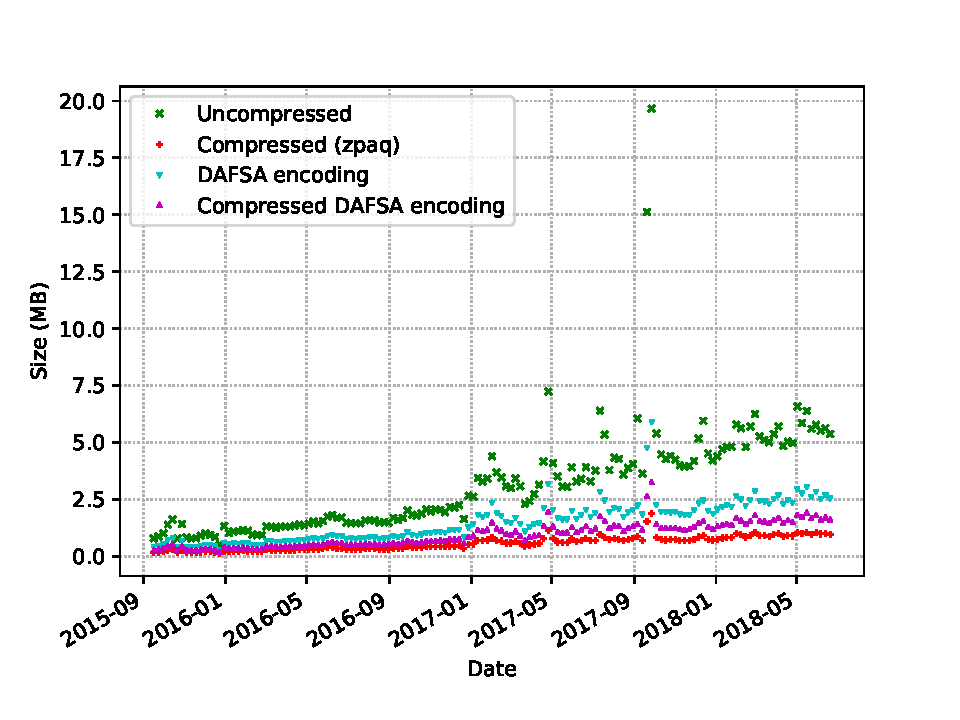
\includegraphics[width=\linewidth]{fig/deleted_name_set_size}
  \label{fig:updates:deleted}
  \caption{Size of deleted names sets over time.}
\end{figure}

\begin{figure}[t]
  \centering
  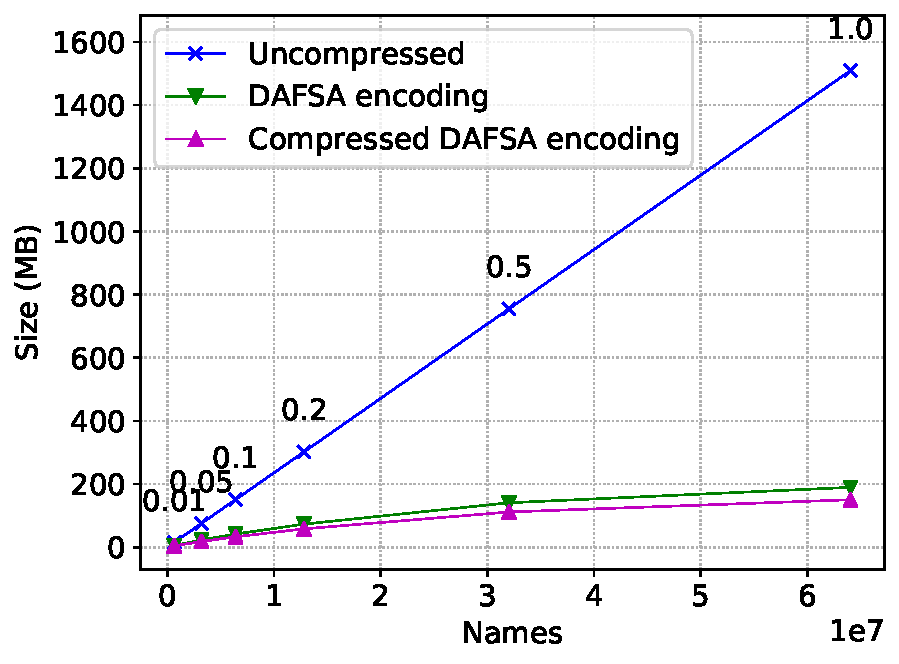
\includegraphics[width=\linewidth]{fig/sample}
  \caption{Size of the signaling set in various representations when 
           the names in the set are subsampled from the full set of names. 
           The labels above each distinct value on the $x$-axis
           denote the fraction of the full set that was sampled.}
  \label{fig:sample}
\end{figure}

\begin{figure}[t]
  \centering
  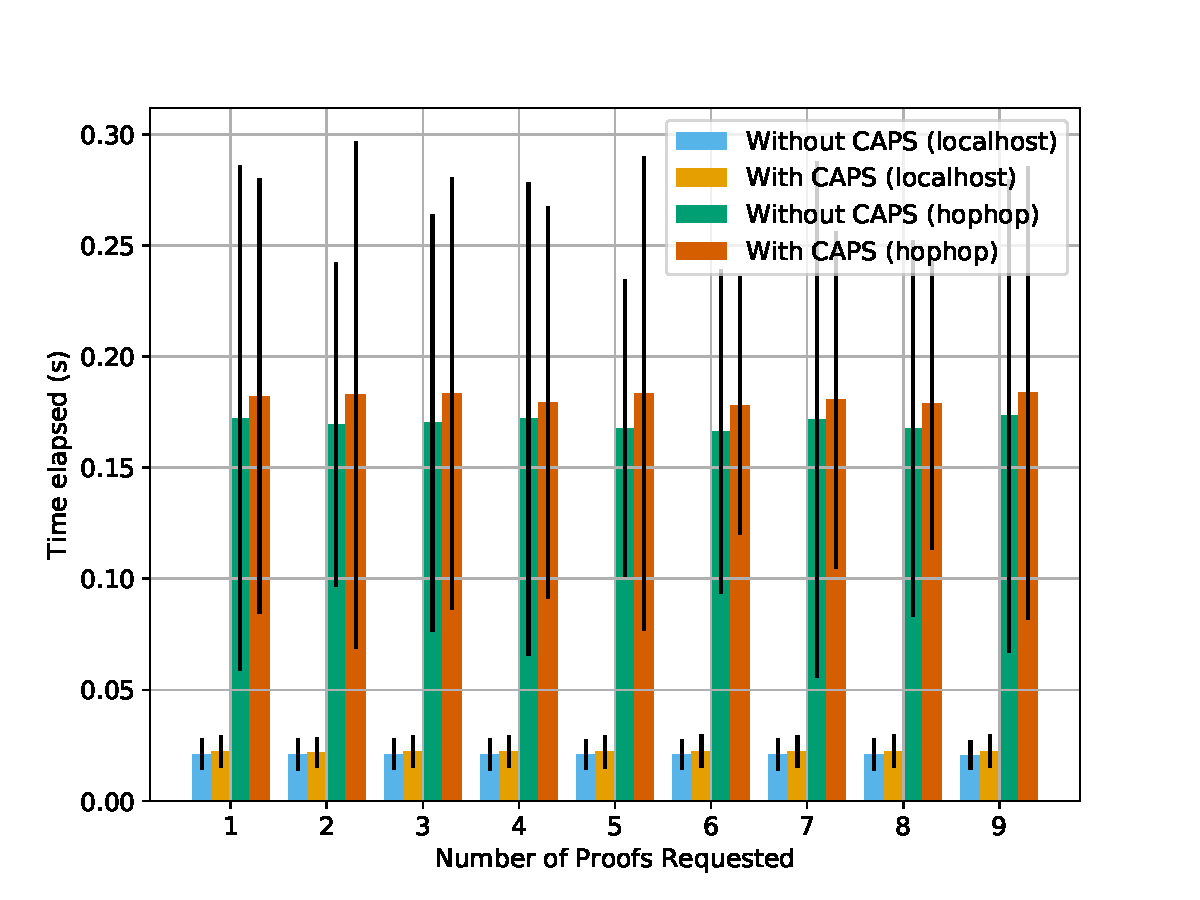
\includegraphics[width=\linewidth]{fig/eval_tls_ext/0-time_elapsed_vs_num_proofs_requested}
  \caption{Handshake latency versus the number of policy proofs sent by the
  domain. Error bars represent standard error.}
  \label{fig:numproofs}
\end{figure}

\begin{figure}[t]
  \centering
  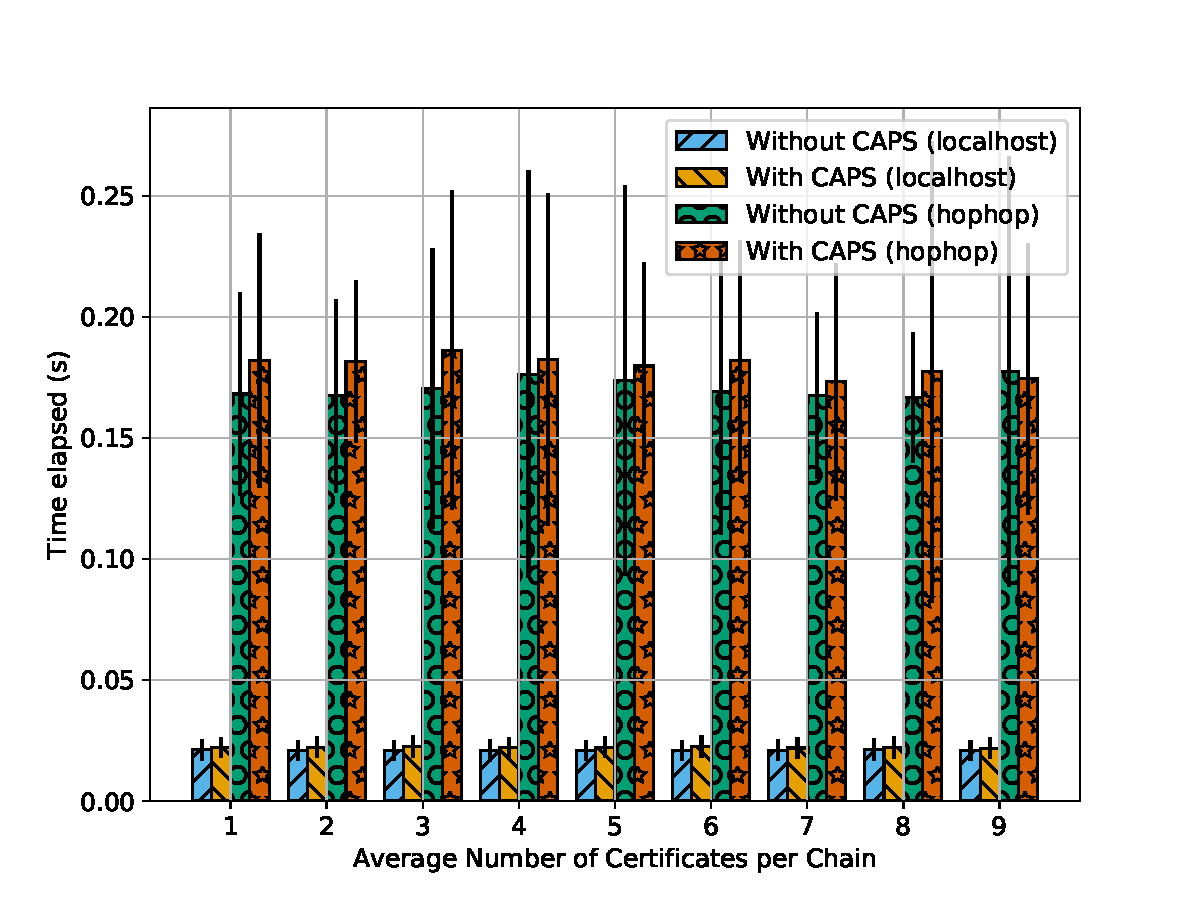
\includegraphics[width=\linewidth]{fig/eval_tls_ext/2-time_elapsed_vs_num_certs_per_chain}
  \caption{Handshake latency versus the number of certificates per chain sent by the
  domain. Error bars represent standard error.}
  \label{fig:numcerts}
\end{figure}

\begin{figure}[t]
  \centering
  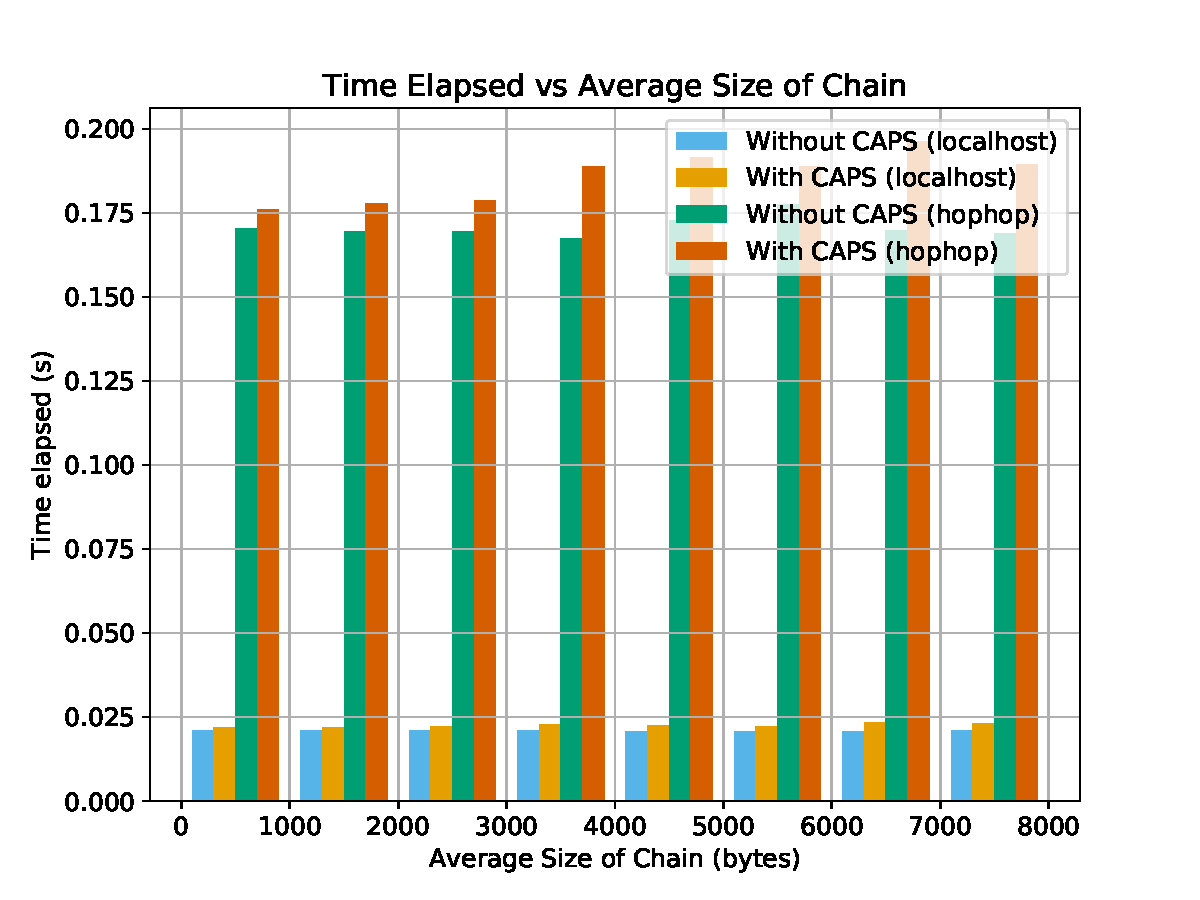
\includegraphics[width=\linewidth]{fig/eval_tls_ext/3-time_elapsed_vs_avg_chain_size}
  \caption{Handshake latency versus the average certificate chain size sent by the
  domain. Error bars represent standard error.}
  \label{fig:chainsize}
\end{figure}

The extra data sent in the \ac{name} handshake is directly dependent on the size
and number of certificate chains, as well as the number of proofs sent. In
particular, the extra data sent from client to server is 1 byte, and the extra
data sent from server to client is
$(2 + (292 \times \text{\#proofs}) +
(\sum_{\text{chain}}\texttt{sizeof}(\text{chain})))$ bytes. 

\paragraph{Data Source Integrity}

\ac{name} relies on the integrity of the data sources (in our current prototype,
Censys and \ac{ct}). Therefore, \iac{ca} who issues
and publicizes an unauthorized certificate for a domain that does not deploy
\ac{https} can cause the domain to be included in the signal set and thus render
the domain inaccessible. This fragility effectively allows an adversary who controls
one or more private CA keys to
``poison the well'' that \ac{name} relies on, and execute a denial-of-service
attack with just a single unauthorized certificate.

To recover from such an attack, the
affected domain could request that the \ac{ca} revoke the certificate if the
\ac{ca} issued the certificate in error. If the \ac{ca} deliberately misissued
the certificate, the browser vendor could treat the certificate as revoked
(though such action is unlikely unless the domain is popular). The affected
domain could also upgrade to \ac{https}, obtaining enough certificates to
override the misissued certificate. 
%In the event that the domain wishes to
%remain without \ac{https}, we can allow domains to set a policy flag that
%signals that the domain will communicate over HTTP. The domain, however, must
%still send this policy and proof during connection establishment.

Enhancements to certificate logs to mitigate situations such as this are ongoing. Some
\ac{ct} logs, for example, only accept certificates from certain \acp{ca}, and
nearly all of them perform some level of certificate validation, including
checking whether a certificate is anchored in a known root certificate. We
expect an attack that involves poisoning data sources in this way to be possible
but rare and noticeable, and an attacker seeking to carry out \iac{mitm} in this way has a
higher hurdle for the attack to succeed than in today's Web \ac{pki}.

\paragraph{Increasing \ac{https} Adoption}

In the past several years, Let's Encrypt and similar efforts to increase
the use of \ac{https} in the Internet has caused a marked increase in the number
of domain names served over \ac{tls}, as shown in
\autoref{sec:evaluation:https}. Due to the structure of DNS, it is impossible to
know how many domain names there are overall, and thus difficult to determine a
ceiling for the number of names known to serve content over \ac{https}.
Therefore, it is possible that the signaling set may grow to a size that is
untenable for increasingly many clients.
However, this may also be offset by the upward trend in available bandwidth
(e.g., the upcoming move to 5G).
We could also mitigate the memory and disk usage for clients by splitting the 
signaling set into several \ac{dafsa} representations based 
on a client's region or self-selected categories of interest.
We also considered splitting the DAFSA based on popularity,
but conversations with Mozilla indicate this approach is not palatable
as it is seen as perpetuating inequality on the Web;
hence any solution should ideally treat websites large and small 
in an egalitarian fashion~\cite{privatecomm}.

\paragraph{Future Work}

One avenue of future exploration that is currently ongoing is \emph{transition
compaction}, which aims to minimize our \ac{dafsa} representation by reducing
the representation size of each transition. A transition in the representation
consists of a symbol and destination state. We have found that in the current
signaling set representation, the symbols and destination states had a
long-tailed distribution. Thus by using variable-length encodings, we can reduce
the overall size of each transition. One straightforward way to do so is via
Huffman encoding, but the long-tailed distribution results in a Huffman
dictionary whose size is significant enough to neutralize any space savings that
would result. We are currently exploring heuristics by which we can select a
subset of symbols to Huffman encode (such as ones that occur more than a
threshold number of times). For destination states, we can assign an ordering of
states in the \ac{dafsa} such that the difference to each destination state in
the ordering is small, and we can then use integer encoding to represent the
location of these states. We are currently exploring the possibility of using
graph vertex separators to address this problem.

%We also plan to examine the use of multiple \acp{dafsa}, collecting data on
%domain names including relative popularity, region, and category. We can then
%construct multiple \ac{dafsa} according to our existing approach, and evaluate
%disk space, memory usage, and connection latency (particularly if we dynamically
%load \acp{dafsa}). We note that some of the necessary data is available from services
%as Alexa Web Information Services and DNS resolvers.

Footnote from 4.2: For efficiency, the log aggregator can sign a subset of pairs
each day, and have each client consider a signature valid for multiple update
intervals. For example, the log aggregator could sign a third of the pairs each
day, and clients could treat a signed, timestamp pair as valid for at least
three days.
